% rsi_71_3_1256-1263:
%  hunspell -l -t ./det_proposal_2015-02-07.tex > sp
%\documentclass[11pt,letterpaper]{article}
\documentclass[10pt]{revtex4}
%\usepackage{pictex}
%\usepackage[dvips]{epsfig}
\usepackage{graphicx}
\usepackage{url}
\usepackage{braket}
\usepackage{amssymb}
\usepackage{amsmath}
\setlength{\unitlength}{1mm}
\setlength{\evensidemargin}{-1cm}
\setlength{\oddsidemargin}{-1cm}
%\addtolength{\topmargin} {-2cm}
\setlength{\textwidth}{17.5cm}
%\setlength{\textheight}{23.5cm}
\renewcommand{\topfraction}{1}
\renewcommand{\textfraction}{0}
\setcounter{topnumber}{4}
\setcounter{totalnumber}{5}
%\parindent 1.5mm
%\input mytexinp.tex
\def\bfm#1{{\bf #1}}
\def\ra{\rightarrow}
\def\cd{\cdot}
\def\bA{\bfm{A}}
\def\bB{\bfm{B}}
\def\bE{\bfm{E}}
\def\bH{\bfm{H}}
\def\be{\bfm{e}}
\def\bk{\bfm{k}}
\def\bko{\bfm{k}_0}
\def\bkh{\bfm{k}_h}
\def\bkH{\bfm{k}_H}
\def\bp{\bfm{p}}
\def\bq{\bfm{q}}
\def\br{\bfm{r}}
\def\bu{\bfm{u}}
\def\bv{\bfm{v}}
\def\bx{\bfm{x}}
\def\b0{\bfm{0}}
\def\geka{Ge K$_{\alpha_1}$}
\def\bo{\bfm{0}}
\def\gekat{Ge K$_{\alpha_2}$}
\def\bs{\mbox{$\backslash$}}
\def\SetFigFont#1#2#3{}
\def\figbox#1{\fbox{#1}}
\def\C3PO{{C$^3$PO}}
\pagestyle{myheadings}
%\markright{version 1.1 of \today}
\begin{document}
%\markright{file instr\_pro\_8\_04.tex of \today}
\title{C$^3$PO}
\vspace{4mm}
\par
\author{Bernhard W.\ Adams, \today}
%\begin{abstract}
%\end{abstract}
\maketitle
%%%%%%%%%%%%
%\section{Introduction}
%%%%%%%%%%%%%%%%%%%%%%%%%%%%%%%%%%%%%%%%%%%%%%
%%%%%%%%%%%%%%%%%%%%%
\section{Introduction}
\label{s_intro}
\C3PO (Control Code Collection for Process Organization) is a 
system of python scripts that interface industrial-control devices
to a user.
The python scripts can be accessed from the command line, through
operating-system calls, or a GUI (if someone cares to write one).
All implementation-specific information is contained in a PostgreSQL
database.
\par
Experiment control can be abstracted as 1) converting real-world items
of interest to data (numeric, string, image, etc.), 2) processing the
data in a program, and 3) converting data to a real-world effect.
A good approach is to layer the control software into low-level drivers
that interface with a hardware-abstracted (HA) control software, which
allows scripting in any number of levels.
Scripting can be done on the level of the operating system, i.e.,
though system calls.
The interface between the low-level drivers and the lowest
hardware-abstracted software needs to be standardized, yet flexible.
In C$^3$PO, the real world is abstracted though process variables (PVs)
that the lowest HA layer reads from and writes to.
Data formats of PVs can be numeric, string, or vectors or matrices of these.
When a PV is used (written to or read form), the lowest-level HA
program looks up the PV name in the database to find the following
information:
\begin{itemize}
\item name of the driver program, as known to the OS command line
\item type: read/write/other. If an invalid operation is attempted,
for example, writing to a read-only PV,
then an error message is generated, and nothing more happens
\item optional side effect: the name of an OS-command-line program
that may do other things. This may sound rather harmless at first,
but it may be used to
ensure database consistency (see below), or for advanced operations,
such as sending an email message if a motor is moved, or measured
value exceeds a threshold
\end{itemize}
\par
Drivers are python scripts that can be executed from the command line.
Users should never access drivers directly, but only through
the HA layer structure.


%%%%%%%%%%%%%%%
\section{Structure}
\label{s_str}
\C3PO has a layered structure with lower-level, hardware-specific, 
and higher-level user routines, all of which access a database for
specific information, such as PV definitions.
A schematic of the structure is shown in Fig.\ \ref{s_str:f_str}.
%%%%%%%%%%%%%%%%
\begin{figure}
\figbox{
\begin{picture}(170,95)
\put(0,0){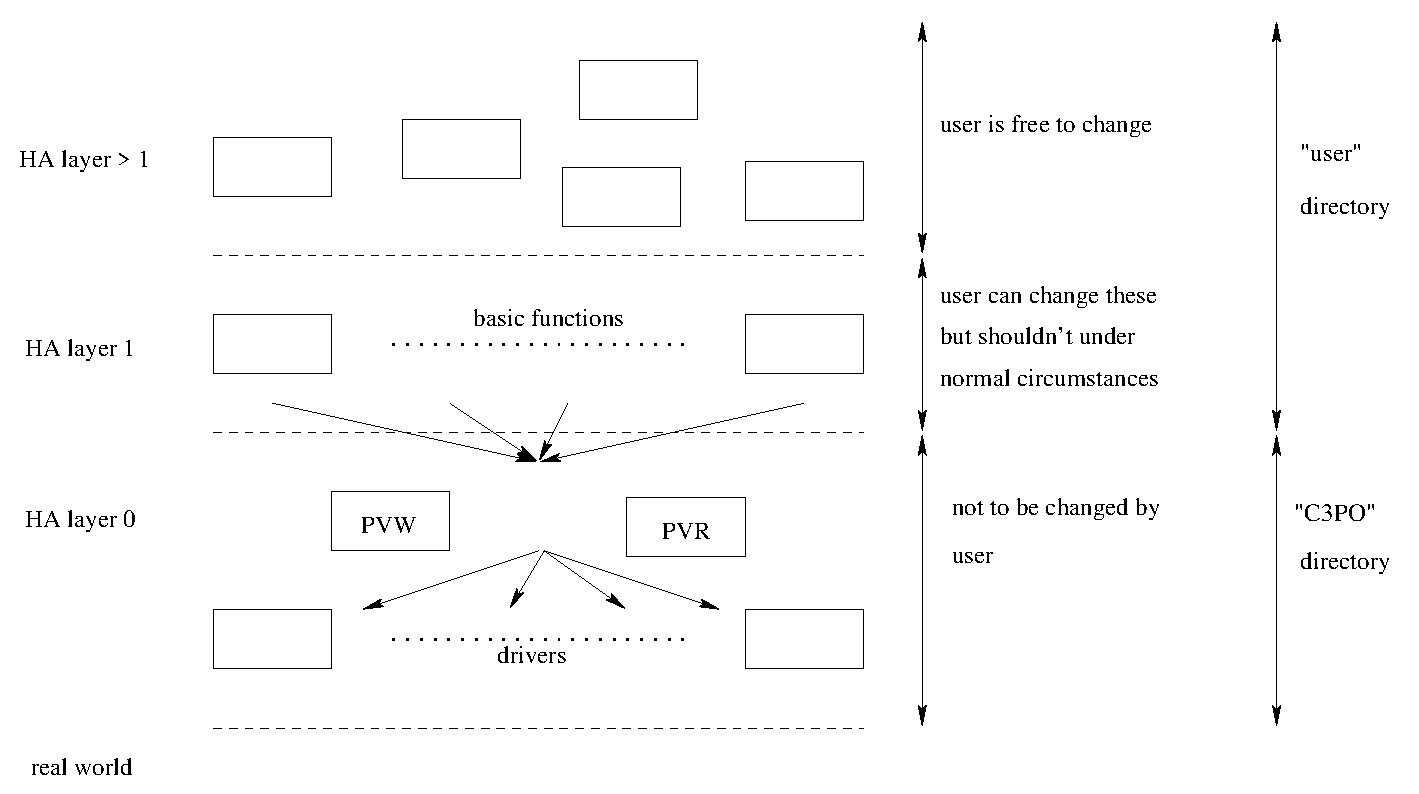
\includegraphics[scale=0.7]{structure.eps}}
\end{picture}
}
\caption{\label{s_str:f_str}Layered structure of C3PO. Higher-level
functions call lower-level ones. All commands flow through the
constriction of a few level-1 scripts calling only two level-0 scripts
(see text).}
\end{figure}
%%%%%%%%%%%%%%%%
Above the level of drivers lies hardware-abstraction layer 0 (HA0),
which, currently, consists of only two scripts, pvw.py for writing to
a PV and pvr.py for reading from a PV.
The drivers and HA0 scripts reside in a dedicated directory called
``C3PO'' in this text.
HA1 and above reside in a ``user'' directory.
In the user directory, there is a file called ``database'', whcih
contains a single line with the name of the database.
By changing that name, a user can easily change the way that the user
scripts interface with the rest of the system.
It is recommended that users do not change the HA1 scripts in the user
directory because these are the standard interfaces to the HA0 scripts in
the C3PO directory.
Instead, user scripts should be at HA level $>1$, and should make
system calls to the HA1 scripts.
\par
The HA1 to HA0 interface between the user and system layers is
constricted to a few HA1 scripts accessing just two HA0 scripts.
This helps to minimize the setup effort, and it also directs the
information flow: Complex operations, such as scans of actuators with
detector readings at each scan point, etc., are reduced to writing
to/reading from PVs.
At that point, re-expansion occurs in another dimension, namely that of
PV names.
\par
The way that a user script interfaces with the real world of the
experiment is as follows:
The user script calls an HA1 script in the user directory and passes
information (for example a target position of an actuator, or a
request to read a voltage) to it via command-line parameters.
That HA1 script determines a PV name or an alias for a PV name
from the command-line information.
Because PVs tend to have somewhat cumbersome names, it is often more
convenient to use an alias, which is resolved by the HA0 scripts (see
below).
PV names or aliases may be passed to an HA1 scripts as a command line
parameter, or they may be implicitly known to the HA1 script,
depending on circumstances.
For example, there may be multiple motors to move in an experiment,
but only one detector to read.
A script named ma to move an actuator (motor) to an
absolute position would need the name of the motor as a command-line
parameter, but in the case of the detector, the name would 
be unnessecary.
The HA1 script then calls the appropriate HA0 script.
If something needs to be moved or changed, then it would call the
script pvw.py with exactly two command-line paramters: the name (or
alias) of the PV to write to, and the value to write.
If a reading needs to be taken, then the script pvr is called with
exactly one argument, then name or alias of the PV to read from, and
the result is returned through the operating system.
The HA0 scripts then try to resolve alias names by looking up the
corresponding PV in a database table called ``alias''.
Then, they consult a database table called ``pvs'' to find the driver
to call for that PV, and finally call the driver with the PV name,
and, in case of a write operation, the value to be written.
Each driver has a database table where the PV name is also entered
with further specific information, such as physical interfaces on the
computer, etc.
%%%%%%%%%%%%%%%
\section{Drivers}
\label{s_drv}
A driver program must accept at least one argument that tells it what
to do, as well as additional optional arguments that depend on the
requested function.
All drivers must support the functions listed in Table.\
\ref{s_drv:t_minf}.


\begin{table}[htb]
\begin{tabular}{|lll|}
\hline
1st argument & returns & format \\
\hline
\hline
ID & ID string & free\\
VER & version & major.minor\\
DATE & date the code was written & yyyy-mm-dd\\
AUT & code author & free\\
DBT & name of table in database & string\\
\hline
\hline
EXEC & & string\\
\hline
\end{tabular}
\caption{\label{s_drv:t_minf}Mandatory (above line) and typical (below
line) functions that a device driver supports.}
\end{table}

%%%%%%%%%%%%%%%
\section{The Database}
The SQL (structured query language) database is a central component of the
control-software suite.
In a small-scale experiment, the database would usually reside on the
same computer that is interfacing with the experiment hardware.
However, it is possible to interface with a database on another
computer on the network.
The database is organized in tables of objects that are abstracted to
have the same structure.
The rows of the table contain the different objects (data items), and
the columns the attributes that are relevant for the objects in the
given context.
The control program uses one mandatory tables
One, called admin, contains some administrative information, most
importantly the directory path where HA Level 0, and below, reside.
The admin table has two columns: key and value.
\par
The other mandatory table is called PVs.
It lists all the PVs used in a given implementation.
The columns in that table are:
\begin{itemize}
\item index no. (integer)
\item PV name (string)
\item type (string)
\item name of driver program (string)
\item execution code for driver (string)
\item optional: name of side-effect program no.\ 1 (string)
\item optional: name of side-effect program no.\ 2 (string)
\item optional: name of side-effect program no.\ 3 (string)
\item optional: name of side-effect program no.\ 4 (string)
\item target value when last accessed (string)
\item actual value when last accessed (string)
\item optional: comment
\end{itemize}
Any additional information that may be needed to use the PV is
contained in the secondary table, the name of which is passed to the
driver, and which the driver knows how to use.
The target and actual values when last accessed are mainly useful
to hold motor positions.
When a value is written to a PV, that value is always entered into the
target value-field.
The actual-value field may be populated from the return value of
side-effect no.\ 1 (if present, see below). 
When a value is read from a PV, that value is always entered into both the
target and actual value fields.
\par
When a PV is accessed, the main HA program looks up the PV name and
checks if the requested operation is compatible with the type (if not,
it exits with an error message).
Then, it looks up the name (to the OS) of the driver program, and passes
the name of the PV, optionally the name of a secondary table where further
information can be found, and the value (in case of a write operation) to the
driver.
The structure of the secondary table depends on the type of PV.
It is usually defined when a new type of PV comes into use, possibly
years after the initial installation.
There are four columns for optinal side-effect programs.
In the unlikely case that more side effects are needed, they must be
handled through indirect calls, i.e., one of the four side effects
calling more, secondary ones.
Side effects may be needed for several reasons.
For example, when a motor is moved to an absolute target position,
there is no guarantee that it will actually reach it.
Then, a side effect could be to call a program that reads back the
actual value.
This function is reserved for side effect no.\ 1



%%%%%%%%%%%%%%%%%%%%%%%%%%
\section{Database Details}
\subsection{Manual Access}
The database can be accessed manually with the command {\tt psql -d xcap}.
It is helpful to do so now and again just to check on how the control
software has modified the database.
Databases that exist for the current user are listed with the command
(on the psql prompt {\tt xcap=>}) $\backslash$d.
The structure of table pvs is displayed with {\tt $\backslash$d pvs;}.
%An entry in the table can be shown with {\tt SELECT }
All entries in table pvs can be shown with {\tt SELECT * from pvs}.
%%%%%%%%%%%%%%%
\subsection{Experiment Setup}
To set up an experiment, one needs to create the database structure.
This could be done manually on the postgrsql prompt, but it would be
a very tedious process.
Instead, one can run a setup python script.
However, to alter an existing setup, for example, to set-up a new
device, mayy be easier to do on the psql command prompt.
\par
Entries into the table are made with the INSERT INTO command at the
database command prompt.
For example,
{\tt INSERT INTO pvs (pvname,type,drname,sectable) VALUES
(`htr.mva', `W', `DCH', `DCH');
}
% https://docs.python.org/3.1/library/subprocess.html
% https://wiki.postgresql.org/wiki/Psycopg2_Tutorial
% https://www.digitalocean.com/community/tutorials/how-to-install-and-use-postgresql-on-ubuntu-14-04
% http://initd.org/psycopg/docs/usage.html
% http://www.tutorialspoint.com/postgresql/postgresql_python.htmhttps://www.digitalocean.com/community/tutorials/how-to-create-remove-manage-tables-in-postgresql-on-a-cloud-server
%
%
%
%%%%%%%%%%%%%
\section{Installation}
\label{s_inst}
System requirements are a contemporary Linux distribution with python
and postgresql software installed. Pyhthon package psycopg
(interface to postgresql) is also required.\\
To install postgresql:\\
{\tt sudo apt-get update}\\
{\tt sudo apt-get install postgresql postgresql-contrib}\\
or use a package-management tool such as synaptic.\\
To install python:\\
{\tt sudo apt-get install python python-psycopg2}
\par
Next, postgresql must be told to give access to the user.
This is done by logging into the postgresql account, which should have
been created automatically upon software installation:\\
log into postgresql account: {\tt sudo -i -u postgres}\\
%open postgresql session: {\tt psql}
allow access: {\tt createuser --interactive}\\
{\tt Enter name of role to add: $<$your user name$>$\\
Shall the new role be a superuser? (y/n) n\\
Shall the new role be allowed to create databases? (y/n) y\\
Shall the new role be allowed to create more new roles? (y/n) n\\
}
Log out of postgresql account {\tt exit}
Create database: {\tt createdb $<$your database name$>$}
\par
Next, the database must be populated with entries.
There are several scripts in the C3PO directory that read the
information from their specific data files and write it to the
respective tables in the database.
These are:\par
%%%%%%%%%%%%%
\begin{tabular}{|llll|}
\hline
script & reads from & writes table & function \\
\hline
\hline
setup\_PVs.py & pvsdefs & pvs & list PV names\\
setup\_alias.py & aliasdefs & alias & create alias names\\
setup\_admin.py & admindefs & admin & administrative stuff (path, etc.)\\

\hline
\end{tabular}
%%%%%%%%%%%%%
\par
It may be helpful to enter a psql session to see interactively what
is going on.
Type at the command line: {\tt psql -d $<$name of database$>$}\\
Then, at the psql prompt:\\
{\tt $\backslash$q} to exit\\
{\tt $\backslash$d} to list tables\\
{\tt $\backslash$d $<$name of table$>$} to list structure of a table\\
{\t select * from $<$name of table$>$} to list all entries in a table\\
The latter is very helpful to see the column names, which are needed
to understand what the scripts are referring to.
%%%%%%%%%%%%%
\section{Example}
Suppose the experiment requires to drive three motors using the
DCH motor controller from Dragonfly Devices, as well as reading
images from a CCD camera, and controlling a temperature.
The motor driver is connected to serial port /dev/ttyUSB0,
the camera requires a call to a program that handles exposure,
readout, etc., and the temperature controller is connected by RS485 bus
to an ethernet-serial bridge.
Assume the motors are called {\tt htr}, {\tt vtr}, and {\tt foc},
and we use a somewhat structured naming convention for the pVs (this
is not necessary, but it is helpful).
For each motor, we want to have PVs to send it to an absolute position,
to a relative position, read back the current position, and read back
the limit-switch status (many more PVs may be desirable).

Then, for each motor, one would require at least PVs to send it to an
absolute position

\bibliographystyle{unsrt}
%\bibliographystyle{apsrev}
\bibliography{phlit,Detectors_2014-10-16}
%\section{Revision history}
%\begin{enumerate}
%\item version: 2014-10-17
%\item version: 2014-10-23, polished intro 
%\end{enumerate}
\end{document}
